\documentclass[aspectratio=169, glossy]{beamer}
\useoutertheme{wuerzburg}
\useinnertheme[realshadow,corners=2pt,padding=2pt]{chamfered}
\usecolortheme{shark}
%%%%%%%%%%%%%%%%%%%%%%%%%%%%%%%%%%%%%%%%%%%%%%%%%%
% PERSONAL STUFF
\usepackage{graphicx}
\usepackage{booktabs}
\usepackage{xcolor}
\usepackage{ulem}

\setlength\abovecaptionskip{-5pt}
\setbeamerfont{footnote}{size=\tiny}
\usepackage[font=footnotesize]{caption}

\usepackage{xcolor}
\definecolor{commentgreen}{RGB}{2,112,10}
\definecolor{eminence}{RGB}{108,48,130}
\definecolor{weborange}{RGB}{255,165,0}
\definecolor{frenchplum}{RGB}{129,20,83}

%%%%%%%%%%%%%%%%%%%%%%%%%%%%%%%%%%%%%%%%%%%%%%%%%%

\newcommand{\backupbegin}{
   \newcounter{finalframe}
   \setcounter{finalframe}{\value{framenumber}}
}
\newcommand{\backupend}{
   \setcounter{framenumber}{\value{finalframe}}
}

%%%%%%%%%%%%%%%%%%%%%%%%%%%%%%%%%%%%%%%%%%%%%%%%%%
\usetikzlibrary{arrows,shapes}
\tikzstyle{every picture}+=[remember picture]
\setbeamertemplate{navigation symbols}{}
% \setbeamertemplate{footline}[frame number]
%\logo{\includegraphics[width= 0.15\linewidth]{full_logo.pdf}\vspace{-9pt}}
\definecolor{MyBlue}{RGB}{33,84,172}
%%%%%%%%%%%%%%%%%%%%%%%%%%%%%%%%%%%%%%%%%%%%%%%%%%%%%%

\title{Capgemini test: forecasting water levels}
\author{Stefano Petrucci}
\institute{}
\date{\today}

\begin{document}

%%%%%%%%%%%%%%%%%%%%%%%%%%%%%%%%%%%%%%%%%%%%%%%%%%%%%%
%%%%%%%%%%%%%%%%%%%%%%%%%%%%%%%%%%%%%%%%%%%%%%%%%%%%%%

\begin{frame}[plain]
\title{\LARGE{\textcolor{MyBlue}{Capgemini test: forecasting water levels}}}
%\subtitle{SUBTITLE}
\author{
	Stefano Petrucci\\
	\footnotesize{petrucci.ste@gmail.com}
% 	{\it University of Edinburgh}\\
}
%\titlegraphic{\includegraphics[width=0.3\textwidth]{plots/full_logo_no_rta.pdf}}
\date{}
% \date{
%     \titlegraphic{\logo}
% 	\\
% 	\vspace{1cm}
% 	\today
% }
\titlepage
% \maketitle
\end{frame}

%%%%%%%%%%%%%%%%%%%%%%%%%%%%%%%%%%%%%%%%%%%%%%%%%%%%%%
%%%%%%%%%%%%%%%%%%%%%%%%%%%%%%%%%%%%%%%%%%%%%%%%%%%%%%

%\begin{frame}
%  \tableofcontents
%\end{frame}

%%%%%%%%%%%%%%%%%%%%%%%%%%%%%%%%%%%%%%%%%%%%%%%%%%%%%%
%%%%%%%%%%%%%%%%%%%%%%%%%%%%%%%%%%%%%%%%%%%%%%%%%%%%%%

\begin{frame}{Data set}
  \begin{columns}
    \begin{column}{0.6\columnwidth}
      \begin{itemize}
        \item Chosen \textit{Lake\_Bilancino}
        \item Two target variables:
          \begin{itemize}
            \item Lake level
            \item Flow rate
          \end{itemize}
        \item Most variables missing before 01/01/2004\\
        $\Rightarrow$ removed since $\sim 9\%$ of the total
        \item Missing data not replaced\footnote{Applied an interpolation only when computing the autocorrelation.}
      \end{itemize}
      \vspace{7em}
    \end{column}
    \begin{column}{0.4\columnwidth}
      \begin{center}
        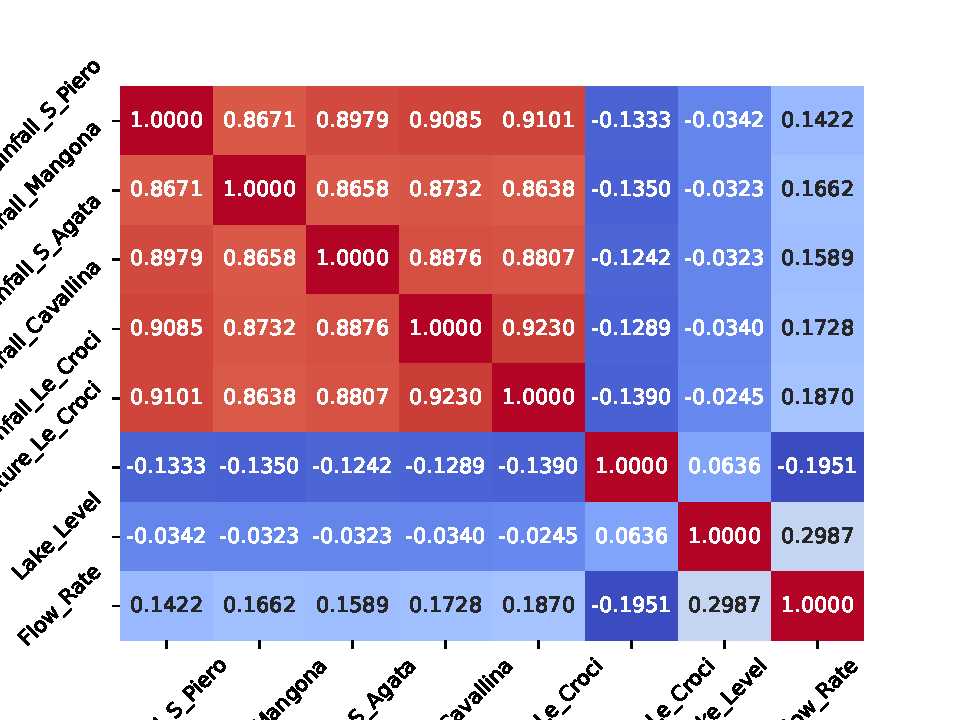
\includegraphics[width=0.8\columnwidth]{../plots/corr_vars.pdf}\\
        \tiny{Covariance matrix}
      \end{center}
    \end{column}
  \end{columns}
\end{frame}

%%%%%%%%%%%%%%%%%%%%%%%%%%%%%%%%%%%%%%%%%%%%%%%%%%%%%%
%%%%%%%%%%%%%%%%%%%%%%%%%%%%%%%%%%%%%%%%%%%%%%%%%%%%%%

\begin{frame}{Forecasting strategy}
  \begin{columns}
    \begin{column}{0.6\columnwidth}
      \begin{enumerate}
          \item Simple AutoRegressive (AR) model
          \item More complex AutoRegressive Integrated Moving Average (ARIMA) model
          \item Multivariate analysis (not implemented)
      \end{enumerate}
    \end{column}
    \begin{column}{0.4\columnwidth}
      \begin{center}
        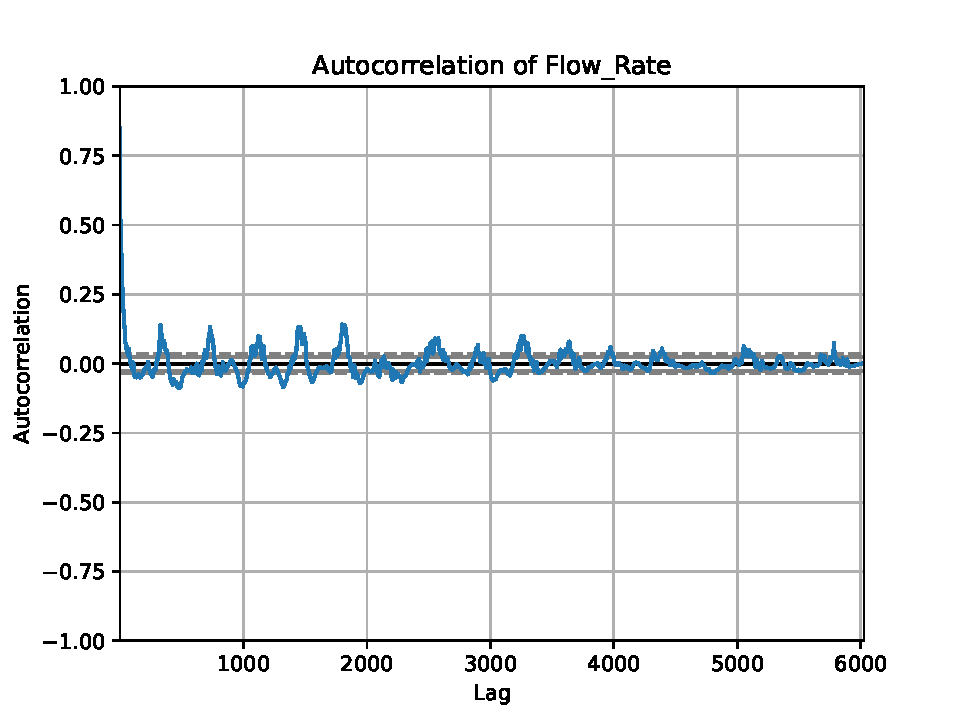
\includegraphics[width=0.65\columnwidth]{../plots/flow_rate_autocorr.pdf}\\
        \tiny{Flow rate - autocorrelation}\\
        \vspace{1em}
        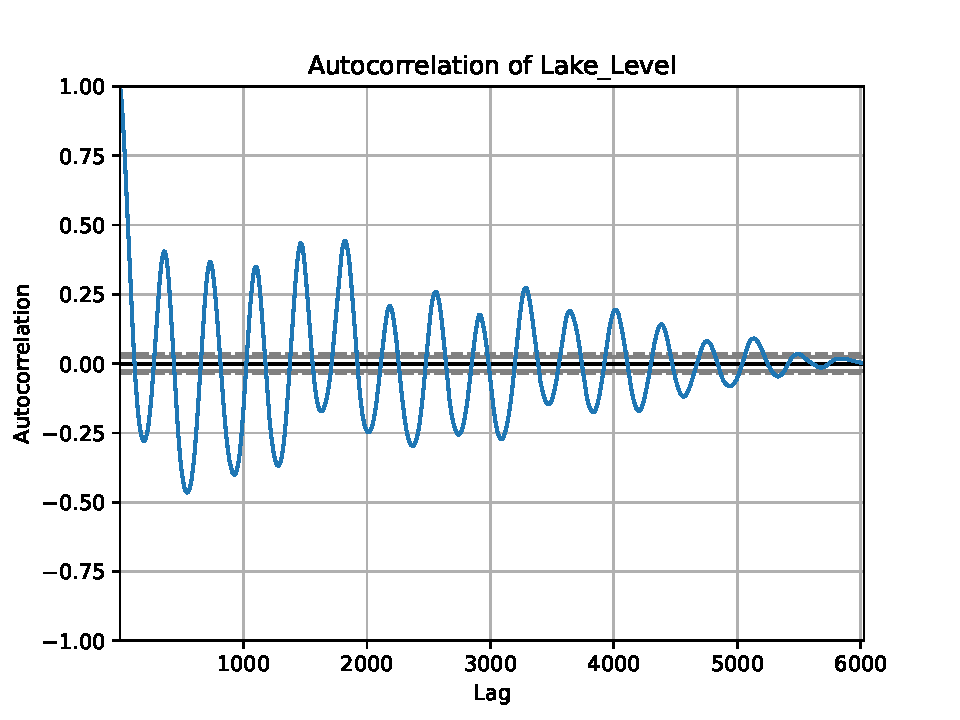
\includegraphics[width=0.65\columnwidth]{../plots/lake_level_autocorr.pdf}\\
        \tiny{Lake level - autocorrelation}
      \end{center}
    \end{column}
  \end{columns}
\end{frame}

%%%%%%%%%%%%%%%%%%%%%%%%%%%%%%%%%%%%%%%%%%%%%%%%%%%%%%
%%%%%%%%%%%%%%%%%%%%%%%%%%%%%%%%%%%%%%%%%%%%%%%%%%%%%%

\begin{frame}{Predictions - 13 samples}
  \begin{columns}
    \begin{column}{0.5\columnwidth}
      \begin{center}
        \vspace{-1em}
        AutoRegressive model\\
        \vspace{0.5em}
        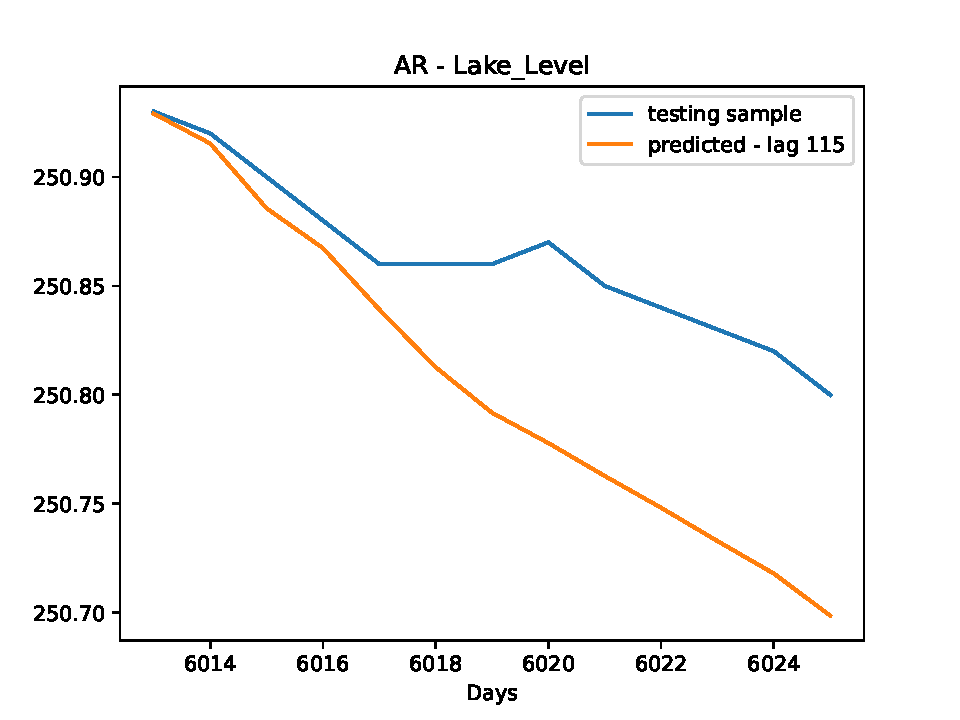
\includegraphics[width=0.5\columnwidth]{../plots/ar_lake_level_prediction.pdf}\\
        \tiny{Lake level}\\
        \vspace{0.5em}
        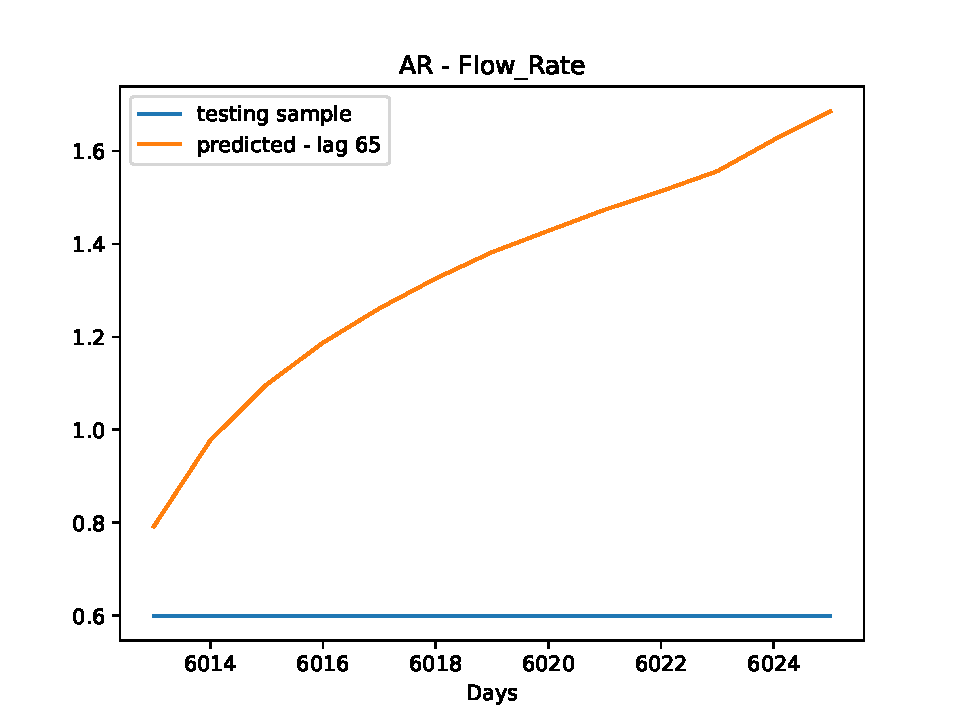
\includegraphics[width=0.5\columnwidth]{../plots/ar_flow_rate_prediction.pdf}\\
        \tiny{Flow rate}
      \end{center}
    \end{column}
    \begin{column}{0.5\columnwidth}
      \begin{center}
        \vspace{-1em}
        ARIMA model\\
        \vspace{0.5em}
        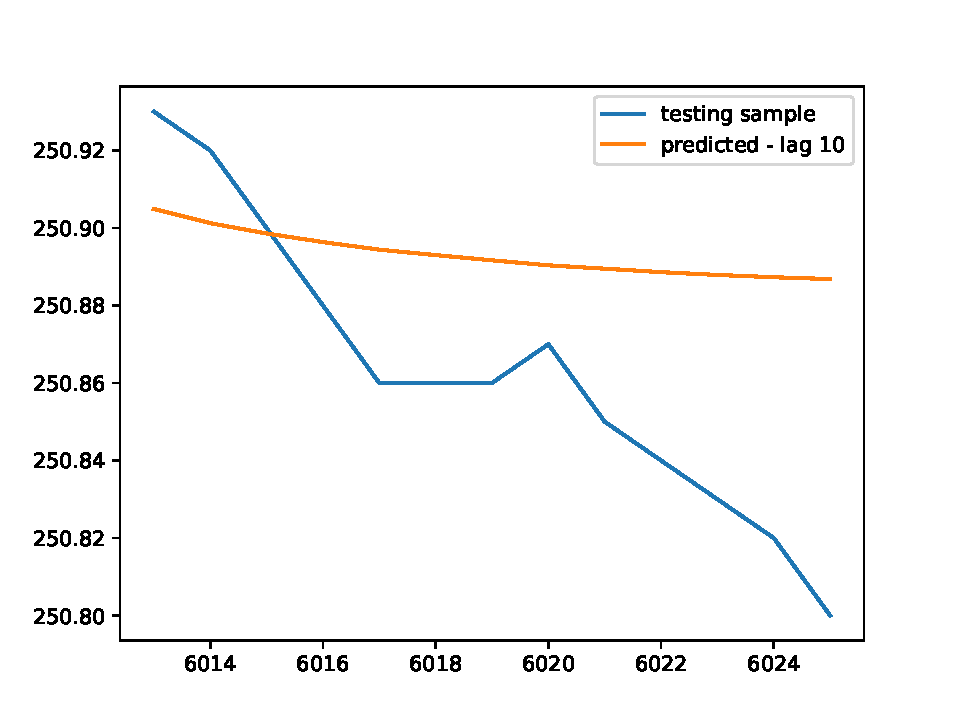
\includegraphics[width=0.5\columnwidth]{../plots/arima_lake_level_prediction.pdf}\\
        \tiny{Lake level}\\
        \vspace{0.5em}
        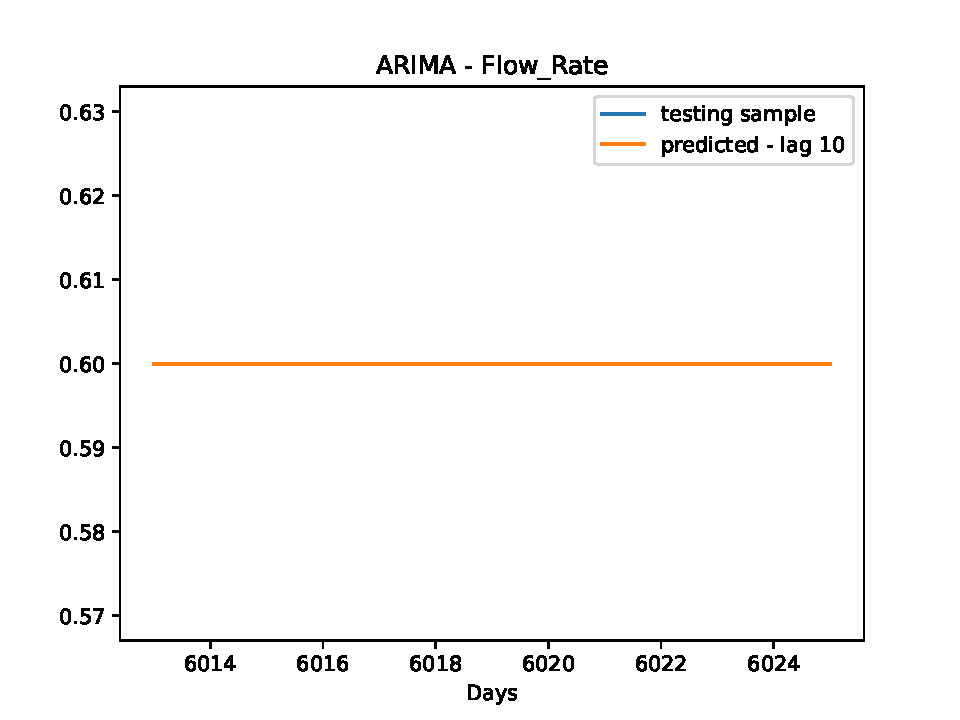
\includegraphics[width=0.5\columnwidth]{../plots/arima_flow_rate_prediction.pdf}\\
        \tiny{Flow rate}
      \end{center}
    \end{column}
  \end{columns}
\end{frame}
%%%%%%%%%%%%%%%%%%%%%%%%%%%%%%%%%%%%%%%%%%%%%%%%%%%%%%
%%%%%%%%%%%%%%%%%%%%%%%%%%%%%%%%%%%%%%%%%%%%%%%%%%%%%%

\begin{frame}{Conclusions}
  \begin{itemize}
    \item 
  \end{itemize}
\end{frame}

%%%%%%%%%%%%%%%%%%%%%%%%%%%%%%%%%%%%%%%%%%%%%%%%%%%%%%
%%%%%%%%%%%%%%%%%%%%%%%%%%%%%%%%%%%%%%%%%%%%%%%%%%%%%%
\end{document}
